
% Monograph LaTeX Template for UFSC based on:
% 1. https://github.com/royertiago/tcc
% 2. http://portal.bu.ufsc.br/normalizacao/
% 3. https://github.com/evandrocoan/ufscthesisx
% 4. http://www.latextemplates.com/template/simple-sectioned-essay

% Initially translated from Portuguese with help of https://github.com/omegat-org/omegat <Computer Assisted Translation of LaTeX document>
% https://tex.stackexchange.com/questions/313732/computer-assisted-translation-of-latex-document

% Allows you to write your thesis both in English and Portuguese
% https://tex.stackexchange.com/questions/5076/is-it-possible-to-keep-my-translation-together-with-original-text
\newif\ifenglish\englishfalse
\newif\ifadvisor\advisorfalse

% Uncomment the line `\englishtrue` to set the document default language to English
% \englishtrue
\advisortrue

% https://tex.stackexchange.com/questions/131002/how-to-expand-ifthenelse-so-that-it-can-be-used-in-parshape
\newcommand{\lang}[2]{\ifenglish#1\else#2\fi}
\newcommand{\advisor}[2]{\ifadvisor#1\else#2\fi}

% https://tex.stackexchange.com/questions/385895/how-to-make-passoptionstopackage-add-the-option-as-the-last
% https://tex.stackexchange.com/questions/484400/changing-the-cleveref-package-language-conjunction-definition
% https://tex.stackexchange.com/questions/516058/why-isnt-my-biblatex-language-changing-when-passing-the-language-on-my-document
\ifenglish
    \PassOptionsToPackage{brazil,main=english,spanish,french}{babel}
\else
    \PassOptionsToPackage{main=brazil,english,spanish,french}{babel}
\fi

% Simple alias for English and Portuguese words
% https://tex.stackexchange.com/questions/513019/argument-of-bbltempd-has-an-extra
\newcommand{\brazilword}[1]{\protect\foreignlanguage{brazil}{#1}}
\newcommand{\englishword}[1]{\protect\foreignlanguage{english}{#1}}

% Allow you to write `Evandro's house` in latex as `Evandro\s house` instead of `Evandro\textquotesingle{}s house`
% https://tex.stackexchange.com/questions/31091/space-after-latex-commands
\newcommand{\s}[0]{\textquotesingle{}s\xspace}
\newcommand{\q}[0]{\textquotesingle{}\xspace}

% Uncomment the following line if you want to use other biblatex settings
% \PassOptionsToPackage{style=numeric,repeatfields=true,backend=biber,backref=true,citecounter=true}{biblatex}
\documentclass[
\lang{english}{brazilian,brazil}, % https://tex.stackexchange.com/questions/484400/changing-the-cleveref-package-language-conjunction-definition
12pt, % Padrão UFSC para versão final
a4paper, % Padrão UFSC para versão final
oneside, % Impressão nos dois lados da folha
chapter=TITLE, % Título de capítulos em caixa alta
section=TITLE, % Título de seções em caixa alta
]{setup/ufscthesisx}

% Utilize o arquivo aftertext/references.bib para incluir sua bibliografia.
% http://tug.ctan.org/tex-archive/macros/latex/contrib/cleveref/cleveref.pdf
\addbibresource{aftertext/references.bib}

% https://www.overleaf.com/learn/latex/Inserting_Images
\graphicspath{{pictures/}}

% FIXME: Preencha com seus dados
\autor{\brazilword{Escreva aqui o Nome completo do Autor ou da Autora}}
\titulo{\lang{Work Title\protect\\Could be break into two lines}{Título do trabalho\protect\\Pode ser Quebrado em duas linhas}}

% FIXME: Se houver subtítulo, descomente a linha abaixo
\subtitulo{\lang{Subtitle}{Subtítulo}}

% FIXME: Siglas para grau de formação Dr./Dra., Me./Ma, Bel. Bela. (inglês: PhD., MSc., Bs.)
\orientador[\lang{Supervisor}{Orientador(a)}]{\brazilword{Nome completo do Orientador(a)}, \lang{Phd.}{Dr.}}

% FIXME: Se houver coorientador, descomente a linha abaixo
% \coorientador[\lang{Co-supervisor}{Coorientador(a)}]{\brazilword{Nome do coorientador(a)}, \lang{Phd.}{Dr.}}

% FIXME: Preencher com o nome do Coordenador de TCCs/Teses do seu curso
\coordenador[\lang{Coordinator}{Coordenador(a)}]{\brazilword{Nome do Coordenador(a)}, \lang{Phd.}{Dr.}}

% FIXME: Local da sua defesa
\local{\brazilword{Florianópolis, Santa Catarina} -- \lang{Brazil}{Brasil}}

% FIXME: Ano da sua defesa
\ano{2019}
\biblioteca{\lang{University Library}{Biblioteca Universitária}}

% FIXME: Sigla da sua instituição
\instituicaosigla{UFSC}
\instituicao{\brazilword{Universidade Federal de Santa Catarina}}

% FIXME: Preencha com Tese, Dissertação, Monografia ou Trabalho de Conclusão de Curso, Bachelor's Thesis, etc
\tipotrabalho{\lang{Bachelor\s Thesis}{Trabalho de Conclusão de Curso}}

% FIXME: Se houver Área de Concentração, descomente a linha abaixo
% \area{\lang{Formal Languages}{Linguagens Formais}}

% FIXME: Preencha com Doutor, Bacharel ou Mestrando
\formacao{\lang
    {Bachelor of Science degree in Computer Science}
    {Bacharel em Ciências da Computação}%
}
\programa{\lang
    {Undergraduate Program in Computer Science}
    {Programa de Graduação em Ciências da Computação}%
}

% FIXME: Preencha com Departamento de XXXXXX, Centro de XXXXXX
\centro{\lang
    {INE -- Department of Informatics and Statistics, CTC -- Technological Center}
    {INE -- Departamento de Informática e Estatística, CTC -- Centro Tecnológico}%
}

% FIXME: Preencha com Campus XXXXXX     ou     Centro de XXXXXX
\campus{\brazilword{Campus Reitor João David Ferreira Lima}}

% FIXME: Data da sua defesa
\data{\lang{30 of march of}{30 de março de} 2019}

% O preambulo deve conter tipo do trabalho, objetivo, nome da instituição e a área de concentração.
\preambulo{\lang%
    {%
        \imprimirtipotrabalho~submitted to the \imprimirprograma~of
        \imprimirinstituicao~for degree acquirement in \imprimirformacao.%
    }{%
        \imprimirtipotrabalho~submetido ao \imprimirprograma~da
        \imprimirinstituicao~para a obtenção do Grau de \imprimirformacao.%
    }%
}

% Allows you to use ~= instead of `\hyp{}`
% https://tex.stackexchange.com/questions/488008/how-to-create-an-alternative-to-shortcut-or-hyp
% https://tex.stackexchange.com/questions/405718/depending-on-babel-language-setting-i-get-biblatex-error-argument-of-language
% https://tex.stackexchange.com/questions/340661/argument-of-languageactivearg-has-an-extra-i-use-includegraphics-and-r
\useshorthands{~}\defineshorthand{~=}{\hyp{}}

\palavraschaveufsc{palavraschaveingles}   {Keyword 1}
\palavraschaveufsc{palavraschaveportugues}{Palavra~=Chave 1}

\palavraschaveufsc{palavraschaveingles}   {Keyword 2}
\palavraschaveufsc{palavraschaveportugues}{Palavra~=Chave 2}

\palavraschaveufsc{palavraschaveingles}   {Keyword 3}
\palavraschaveufsc{palavraschaveportugues}{Palavra~=Chave 3}


\hypersetup
{
    pdfsubject={Thesis' Abstract},
    pdfcreator={LaTeX with abnTeX2 for UFSC},
    pdftitle={\imprimirtitulo},
    pdfauthor={\imprimirautor},
    pdfkeywords={\lang{\palavraschaveinglessemitem}{\palavraschaveportuguessemitem}},
}

% Altere o arquivo 'settings.tex' para incluir customizações de aparência da sua tese
%----------------------------------------------------------------------------------------
%   Thesis Tweaks and Utilities
%----------------------------------------------------------------------------------------
\makeatletter


% Uncomment this if you are debugging pages' badness Underfull & Overflow
% https://tex.stackexchange.com/questions/115908/geometry-showframe-landscape
% https://tex.stackexchange.com/questions/387077/what-is-the-difference-between-usepackageshowframe-and-usepackageshowframe
% https://tex.stackexchange.com/questions/387257/how-to-do-the-memoir-headings-fix-but-not-have-my-text-going-over-the-page-botto
% https://tex.stackexchange.com/questions/14508/print-page-margins-of-a-document
% \usepackage[showframe,pass]{geometry}

% To use the font Times New Roman, instead of the default LaTeX font
% more up-to-date than '\usepackage{mathptmx}'
% \usepackage{newtxtext}
% \usepackage{newtxmath}

% https://tex.stackexchange.com/questions/182569/how-to-manually-set-where-a-word-is-split
\hyphenation{Ge-la-im}
\hyphenation{Cis-la-ghi}

% Add missing translations for Portuguese
% https://tex.stackexchange.com/questions/8564/what-is-the-right-way-to-redefine-macros-defined-by-babel
\@ifpackageloaded{babel}{\@ifpackagewith{babel}{brazil}{\addto\captionsbrazil{%
  \renewcommand{\mytextpreliminarylistname}{Breve Sumário}
}}{}}{}
\@ifundefined{advisor}{\newcommand{\advisor}[2]{#1}}{}

% Selects a sans serif font family
% \renewcommand{\sfdefault}{cmss}

% Selects a monospaced (“typewriter”) font family
% \renewcommand{\ttdefault}{cmtt}

% Spacing between lines and paragraphs
% https://tex.stackexchange.com/questions/70212/ifpackageloaded-question
\@ifclassloaded{memoir}
{
  % New custom chapter style VZ14, see other chapters styles in:
  % http://repositorios.cpai.unb.br/ctan/info/latex-samples/MemoirChapStyles/MemoirChapStyles.pdf
  \newcommand\thickhrulefill{\leavevmode \leaders \hrule height 1ex \hfill \kern \z@}
  \makechapterstyle{VZ14} { %
    % \thispagestyle{empty}
    \setlength\beforechapskip{50pt}
    \setlength\midchapskip{20pt}
    \setlength\afterchapskip{20pt}
    \renewcommand\chapternamenum{}
    \renewcommand\printchaptername{}
    \renewcommand\chapnamefont{\Huge\scshape}
    \renewcommand\printchapternum {%
      \chapnamefont\null\thickhrulefill\quad
      \@chapapp\space\thechapter\quad\thickhrulefill
    }
    \renewcommand\printchapternonum {%
      \par\thickhrulefill\par\vskip\midchapskip
      \hrule\vskip\midchapskip
    }
    \renewcommand\chaptitlefont{\huge\scshape\centering}
    \renewcommand\afterchapternum {%
      \par\nobreak\vskip\midchapskip\hrule\vskip\midchapskip
    }
    \renewcommand\afterchaptertitle {%
      \par\vskip\midchapskip\hrule\nobreak\vskip\afterchapskip
    }
  }

  % Apply the style `VZ14` just created
  % \chapterstyle{VZ14}

  % http://mirrors.ibiblio.org/CTAN/macros/latex/contrib/memoir/memman.pdf
  \setlength\beforechapskip{0pt}
  \setlength\midchapskip{15pt}
  \setlength\afterchapskip{15pt}

  % Memoir: Warnings “The material used in the headers is too large” w/ accented titles
  % https://tex.stackexchange.com/questions/387293/how-to-change-the-page-layout-with-memoir
  \setheadfoot{30.0pt}{\footskip}
  \checkandfixthelayout
}{}

% Controlling the spacing between one paragraph and another
% Default value for UFSC 0.0cm
\setlength{\parskip}{\advisor{0.0cm}{0.2cm}}

% Paragraph size is given by
% Default value for UFSC 1.5cm
% \setlength{\parindent}{1.3cm}

% https://tex.stackexchange.com/questions/148647/how-to-remove-space-before-enumerate
% https://tex.stackexchange.com/questions/433543/behaviour-of-enumitem-setlist
\advisor{}{
    \setlist*[enumerate]{label=\arabic*,}
    \setlist*[enumerateoptional]{label=\arabic*,}

    % https://tex.stackexchange.com/questions/24454/space-after-float-with-h
    % https://tex.stackexchange.com/questions/23313/how-can-i-reduce-padding-after-figure
    \AtBeginEnvironment{figure}{
      \setlength{\intextsep}{5pt} % Vertical space above & below [h] floats
      % \setlength{\textfloatsep}{10pt} % Vertical space below (above) [t] ([b]) floats
      % \setlength{\abovecaptionskip}{10pt}
      % \setlength{\belowcaptionskip}{5pt}
    }

    % Patch the `abntex2` citacao environment removing the extra space from its top
    % https://tex.stackexchange.com/questions/300340/topsep-itemsep-partopsep-and-parsep-what-does-each-of-them-mean-and-wha
    \xpatchcmd{\citacao}
    {\list{}}
    {\list{}{\topsep=0pt}}
    {}
    {\FAILEDPATCHINGCITACAO}
}


% Color settings across the document
\@ifpackageloaded{xcolor}
{
  % RGB colors in absolute values from 0 to 255 by using `RGB` tag
  \definecolor{darkblue}{RGB}{26,13,178}

  % Colors names definitions as RGB colors in percentage notation by using `rgb` tag
  \definecolor{mygreen}{rgb}{0,0.6,0}
  \definecolor{mygray}{rgb}{0.5,0.5,0.5}
  \definecolor{mymauve}{rgb}{0.58,0,0.82}
  \definecolor{figcolor}{rgb}{1,0.4,0}
  \definecolor{tabcolor}{rgb}{1,0.4,0}
  \definecolor{eqncolor}{rgb}{1,0.4,0}
  \definecolor{linkcolor}{rgb}{1,0.4,0}
  \definecolor{citecolor}{rgb}{1,0.4,0}
  \definecolor{seccolor}{rgb}{0,0,1}
  \definecolor{abscolor}{rgb}{0,0,1}
  \definecolor{titlecolor}{rgb}{0,0,1}
  \definecolor{biocolor}{rgb}{0,0,1}
  \definecolor{blue}{RGB}{41,5,195}

  % PDF Hyperlinks settings
  \@ifpackageloaded{hyperref}
  {
    \hypersetup
    {
      colorlinks=true,     % false: boxed links; true: colored links
      linkcolor=darkblue,  % color of internal links
      citecolor=darkblue, % color of links to bibliography
      filecolor=black,     % color of file links
      urlcolor=\advisor{black}{darkgreen},
      bookmarksdepth=4,
      pdfencoding=auto,%
      psdextra,
    }
  }
}{}


% Filtering and Mapping Bibliographies
% \DeclareFieldFormat{url}{Disponível~em:\addspace\url{#1}}

% https://tex.stackexchange.com/questions/517526/how-to-make-biblatex-url-links-generated-with-brackets-around-it-url-correctly
\DeclareFieldFormat{url}{\bibstring{urlfrom}\addcolon\space\textless\url{#1}\textgreater}
\DefineBibliographyStrings{brazil}{urlfrom = {Disponível em}}
\DefineBibliographyStrings{english}{urlfrom = {Available from}}

% https://tex.stackexchange.com/questions/391695/is-possible-to-remove-the-link-color-of-the-comma-on-the-citation-link
% \DeclareFieldFormat{citehyperref}{#1}

% % https://tex.stackexchange.com/questions/203764/reduce-font-size-of-bibliography-overfull-bibliography
% \newcommand{\bibliographyfontsize}{\fontsize{10.0pt}{10.5pt}\selectfont}
% \renewcommand*{\bibfont}{\bibliographyfontsize}

% Uncomment this to insert the abstract into your bibliography entries when the abstract is available
% https://tex.stackexchange.com/questions/398666/how-to-correctly-insert-and-justify-abstract
\ifadvisor
\else
  \DeclareFieldFormat{abstract}%
  {%
    \par\justifying
    \begin{adjustwidth}{1cm}{}
      \textbf{\bibsentence\bibstring{abstract}:} #1
    \end{adjustwidth}
  }
  \renewbibmacro*{finentry}%
  {%
    \iffieldundef{abstract}
    {\finentry}
    {\finentrypunct
      \printfield{abstract}%
      \renewcommand*{\finentrypunct}{}%
      \finentry
    }
  }

  % Backref package settings, pages with citations in bibliography
  \newcommand{\biblatexcitedntimes}{\autocap{c}ited \arabic{citecounter} times}
  \newcommand{\biblatexcitedonetime}{\autocap{c}ited one time}
  \newcommand{\biblatexcitednotimes}{\autocap{n}o citation in the text}

  \@ifpackageloaded{babel}{\@ifpackagewith{babel}{brazil}{\addto\captionsbrazil{%
    \renewcommand{\biblatexcitedntimes}{\autocap{c}itado \arabic{citecounter} vezes}
    \renewcommand{\biblatexcitedonetime}{\autocap{c}itado uma vez}
    \renewcommand{\biblatexcitednotimes}{\autocap{n}enhuma citação no texto}
  }}{}}{}
  \@ifpackageloaded{biblatex}
  {%
    % https://tex.stackexchange.com/questions/483707/how-to-detect-whether-the-option-citecounter-was-enabled-on-biblatex
    \ifx\blx@citecounter\relax
      \message{Is citecounter defined? NO!^^J}
    \else
      \message{Is citecounter defined? YES!^^J}
      \ifbacktracker
        \message{Is backtracker defined? YES!^^J}
        \renewbibmacro*{pageref}
        {%
          % https://tex.stackexchange.com/questions/516054/how-to-use-a-dot-to-separate-my-new-bibliography-entry
          \renewcommand*{\bibpagerefpunct}{\addperiod\space}%
          \iflistundef{pageref}%
          {\printtext{\biblatexcitednotimes}}
          {%
            \printtext
            {%
              \ifnumgreater{\value{citecounter}}{1}
                {\biblatexcitedntimes}
                {\biblatexcitedonetime}%
            }%
            \setunit{\addspace}%
            \ifnumgreater{\value{pageref}}{1}
              {\bibstring{backrefpages}\ppspace}
              {\bibstring{backrefpage}\ppspace}%
            \printlist[pageref][-\value{listtotal}]{pageref}%
          }%
        }

        \DefineBibliographyStrings{brazil}
        {
          backrefpage  = {na página},
          backrefpages = {nas páginas},
        }

        \DefineBibliographyStrings{english}
        {
          backrefpage  = {on page},
          backrefpages = {on pages},
        }
      \else
        \message{Is backtracker defined? NO!^^J}
      \fi
    \fi
  }{}
\fi


% https://tex.stackexchange.com/questions/516056/why-an-empty-or-not-biblatex-declaresourcemap-is-removing-my-bibliography-acces
% https://github.com/abntex/biblatex-abnt/pull/56/files
\DeclareStyleSourcemap{%% >>>2
  % This maps some fields used in abntex2cite to biblatex fields.
  \maps[datatype=bibtex]{%
    \map{%
      \step[fieldsource=conference-number,fieldtarget=number]%
      \step[fieldsource=conference-year,fieldtarget=eventdate]%
      \step[fieldsource=conference-location,fieldtarget=venue]%
      \step[fieldsource=conference-number,fieldtarget=number]%
      \step[fieldsource=org-short,fieldtarget=shortauthor]%
      \step[fieldsource=urlaccessdate,fieldtarget=urldate]%
      \step[fieldsource=year-presented,fieldtarget=eventyear]%
      \step[fieldsource=furtherresp,fieldtarget=titleaddon]%
      \step[typesource=journalpart,typetarget=supperiodical]%
    }%
    \map[overwrite=false]{%
      \step[fieldsource=reprinted-from, final]%
      \step[fieldset=related, origfieldval]%
    }%
    \map[overwrite=false]{%
      \step[fieldsource=reprinted-text, final]%
      \step[fieldset=relatedtype, fieldvalue={reprintfrom}]%
    }%
    \map{%
      \pertype{patent}% Use the organization as sourcekey for patents
      \step[fieldsource=organization, final]%
      \step[fieldset=sortkey, origfieldval]%
    }%
    \map[overwrite=false]{%
      \pertype{thesis}%
      \pertype{phdthesis}%
      \pertype{mastersthesis}%
      \pertype{monography}%
      \step[fieldset=bookpagination, fieldvalue={sheet}]%
    }%
    % remove fields that are always useless
    \map{
      % \step[fieldset=abstract, null]
      \step[fieldset=pagetotal, null]
    }
    % % remove URLs for types that are primarily printed
    % \map{
    %   \pernottype{software}
    %   \pernottype{online}
    %   \pernottype{report}
    %   \pernottype{techreport}
    %   \pernottype{standard}
    %   \pernottype{manual}
    %   \pernottype{misc}
    %   \step[fieldset=url, null]
    %   \step[fieldset=urldate, null]
    % }
    \map{
      \pertype{inproceedings}
      % remove mostly redundant conference information
      \step[fieldset=venue, null]
      \step[fieldset=eventdate, null]
      \step[fieldset=eventtitle, null]
      % do not show ISBN for proceedings
      \step[fieldset=isbn, null]
      % Citavi bug
      \step[fieldset=volume, null]
    }
  }%
}% <<<2


% https://tex.stackexchange.com/questions/14314/changing-the-font-of-the-numbers-in-the-toc-in-the-memoir-class
\renewcommand{\cftpartfont}{\ABNTEXpartfont\color{black}}
\renewcommand{\cftpartpagefont}{\ABNTEXpartfont\color{black}}

\renewcommand{\cftchapterfont}{\ABNTEXchapterfont\color{black}}
\renewcommand{\cftchapterpagefont}{\ABNTEXchapterfont\color{black}}

\renewcommand{\cftsectionfont}{\ABNTEXsectionfont\color{black}}
\renewcommand{\cftsectionpagefont}{\ABNTEXsectionfont\color{black}}

\renewcommand{\cftsubsectionfont}{\ABNTEXsubsectionfont\color{black}}
\renewcommand{\cftsubsectionpagefont}{\ABNTEXsubsectionfont\color{black}}

\renewcommand{\cftsubsubsectionfont}{\ABNTEXsubsubsectionfont\color{black}}
\renewcommand{\cftsubsubsectionpagefont}{\ABNTEXsubsubsectionfont\color{black}}

\renewcommand{\cftparagraphfont}{\ABNTEXsubsubsubsectionfont\color{black}}
\renewcommand{\cftparagraphpagefont}{\ABNTEXsubsubsubsectionfont\color{black}}

% Memoir has another mechanism for the job: \cftsetindents{‹kind›}{indent}{numwidth}. Here kind is
% chapter, section, or whatever; the indent specifies the ‘margin’ before the entry starts; and the
% width is of the box into which the number is typeset (so needs to be wide enough for the largest
% number, with the necessary spacing to separate it from what comes after it in the line.
% http://www.tex.ac.uk/FAQ-tocloftwrong.html
% https://tex.stackexchange.com/questions/264668/memoir-indentation-of-unnumbered-sections-in-table-of-contents
% https://tex.stackexchange.com/questions/394227/memoir-toc-indent-the-second-line-by-numberspace
%
% `\cftlastnumwidth` and these `\cftsetindents` are defined by the abntex2 class,
% obeying the `ABNTEXsumario-abnt-6027-2012`. \newlength{\cftlastnumwidth}
% \setlength{\cftlastnumwidth}{\cftsubsubsectionnumwidth}
% \addtolength{\cftlastnumwidth}{-1em}

% http://www.tex.ac.uk/FAQ-tocloftwrong.html
% Use \setlength\cftsectionnumwidth{4em} to override all these values at once
\ifadvisor
\else
  \makechapterstyle{fixedabntex2indentation}
  {%
    \renewcommand{\chapterheadstart}{}
    \setlength{\beforechapskip}{20pt}
    \setlength{\midchapskip}{20pt}
    \setlength{\afterchapskip}{15pt}

    \ifx \chapternamenumlength \undefined
      \newlength{\chapternamenumlength}
    \fi

    % tamanhos de fontes de chapter e part
    \ifthenelse{\equal{\ABNTEXisarticle}{true}}{%
      \setlength\beforechapskip{\baselineskip}%
      \renewcommand{\chaptitlefont}{\ABNTEXsectionfont\ABNTEXsectionfontsize}%
    }{%else
       \setlength{\beforechapskip}{0pt}%
       \renewcommand{\chaptitlefont}{\ABNTEXchapterfont\ABNTEXchapterfontsize}%
    }

    \renewcommand{\chapnumfont}{\chaptitlefont}
    \renewcommand{\parttitlefont}{\ABNTEXpartfont\ABNTEXpartfontsize}
    \renewcommand{\partnumfont}{\ABNTEXpartfont\ABNTEXpartfontsize}
    \renewcommand{\partnamefont}{\ABNTEXpartfont\ABNTEXpartfontsize}

    % tamanhos de fontes de section, subsection, subsubsection e subsubsubsection
    \setsecheadstyle{\ABNTEXsectionfont\ABNTEXsectionfontsize\ABNTEXsectionupperifneeded}
    \setsubsecheadstyle{\ABNTEXsubsectionfont\ABNTEXsubsectionfontsize\ABNTEXsubsectionupperifneeded}
    \setsubsubsecheadstyle{\ABNTEXsubsubsectionfont\ABNTEXsubsubsectionfontsize\ABNTEXsubsubsectionupperifneeded}
    \setsubsubsubsecheadstyle{\ABNTEXsubsubsubsectionfont\ABNTEXsubsubsubsectionfontsize\ABNTEXsubsubsubsectionupperifneeded}

    % Impressão do número do capítulo
    \renewcommand{\chapternamenum}{}

    % Impressão do nome do capítulo
    \renewcommand{\printchaptername}{%
       \chaptitlefont%
       \ifthenelse{\boolean{abntex@apendiceousecao}}{\appendixname}{}%
    }

    % Impressão do título do capítulo
    \def\printchaptertitle##1{%
      \chaptitlefont%
      \ifthenelse{\boolean{abntex@innonumchapter}}{\centering\ABNTEXchapterupperifneeded{##1}}{%
      \ifthenelse{\boolean{abntex@apendiceousecao}}{%
        \centering%
        \settowidth{\chapternamenumlength}{\printchaptername\printchapternum\afterchapternum}%
        \ABNTEXchapterupperifneeded{##1}%
      }{%
        \settowidth{\chapternamenumlength}{\printchaptername\printchapternum\afterchapternum}%
        \parbox[t]{\columnwidth-\chapternamenumlength}{\ABNTEXchapterupperifneeded{##1}}}%
      }%
    }

    % https://tex.stackexchange.com/questions/264668/memoir-indentation-of-unnumbered-sections-in-table-of-contents
    \renewcommand{\tocinnonumchapter}{%
      \addtocontents{toc}{\cftsetindents{chapter}{2.5em}{2em}}%
      \cftinserthook{toc}{A}}

    % Impressão do número do capítulo (no capítulo e não toc)
    \renewcommand{\printchapternum}{%
      \setboolean{abntex@innonumchapter}{false}%
      \chapnumfont%
      ~~\thechapter~%
      \ifthenelse{\boolean{abntex@apendiceousecao}}{%
        \tocinnonumchapter%
        ~\ABNTEXcaptiondelim~~%
      }{}%
    }

    \renewcommand{\ABNTEXcaptiondelim}{~\textendash~}
    \renewcommand{\afterchapternum}{}

    % Impressão do capítulo não numerado
    \renewcommand\printchapternonum{%
      \setboolean{abntex@innonumchapter}{true}%
    }
  }
  \chapterstyle{fixedabntex2indentation}

  \cftsetindents{part}          {0em} {3em}
  \cftsetindents{chapter}       {0em} {3em}
  \cftsetindents{section}       {0em} {4.3em}
  \cftsetindents{subsection}    {0em} {5.2em}
  \cftsetindents{subsubsection} {0em} {5.1em}
  \cftsetindents{paragraph}     {0em} {6.0em}
  \cftsetindents{subparagraph}  {0em} {7.0em}
\fi


\makeatother



% When writing a large document, it is sometimes useful to work on selected sections of the document
% to speed up compilation time: https://en.wikibooks.org/wiki/TeX/includeonly
\newif\ifforcedinclude\forcedincludefalse

% \addtoincludeonly{beforetext/agradecimentos}
% \addtoincludeonly{beforetext/epigrafe}
% \addtoincludeonly{beforetext/fichacatalografica}
% \addtoincludeonly{beforetext/folhadeaprovacao}
% \addtoincludeonly{beforetext/resumos}
% \addtoincludeonly{beforetext/siglas}
% \addtoincludeonly{beforetext/simbolos}

% Part 1
% \addtoincludeonly{chapters/introduction}
% \addtoincludeonly{chapters/motivation}
% \addtoincludeonly{chapters/beautifiers}

% Part 2
\addtoincludeonly{chapters/object_beautifier}
% \addtoincludeonly{chapters/conclusion}
% \addtoincludeonly{aftertext/aftertext}

% Control whether the full document will be generated
% Note: It will also generate severals errors like the following, which can be ignored
%       Latexmk: Missing input file: 'chapters/test.aux'
%
% You can make latex stop generate these errors, if you generate a full version
% of the document, before uncommenting these lines.
%
% Uncomment these two lines, to only partially generate the document
% \doincludeonly
% \forcedincludetrue


% https://tex.stackexchange.com/questions/85113/xrightarrow-text
\makeatletter
\newcommand{\xRightarrow}[2][]{\ext@arrow 0359\Rightarrowfill@{#1}{#2}}
\newcommand{\xLeftarrow}[2][]{\ext@arrow 0359\Leftarrowfill@{#1}{#2}}
\makeatother

% https://tex.stackexchange.com/questions/32208/footnote-runs-onto-second-page
\interfootnotelinepenalty=10000

% Disable the empty pages automatically put by memoir class, except the ones by \cleardoublepage
\ifforcedinclude\openany\else\fi

% https://tex.stackexchange.com/questions/171999/overfull-hbox-in-biblatex
% https://tex.stackexchange.com/questions/499457/why-my-document-is-not-hyphenation-on-words-starting-with-upper-case-letter-i
\emergencystretch=5em

% https://tex.stackexchange.com/questions/23313/how-can-i-reduce-padding-after-figure
% https://tex.stackexchange.com/questions/499580/how-to-keep-my-default-floating-environment-spacing-before-them-while-reducing
% \xpretocmd{\figure}{\setlength{\belowcaptionskip}{-10pt}}{}{}


\begin{document}
    % FIXME: Comment this after finishing the thesis, so you can start fixing the \flushbottom vs \raggedbottom
    % https://tex.stackexchange.com/questions/65355/flushbottom-vs-raggedbottom
    \raggedbottom

    % https://tex.stackexchange.com/questions/4705/double-space-between-sentences
    \frenchspacing

    % Uncomment this to put a ←← | ← (Go To Top/Go Back) on each section header
    \advisor{}{\addGoToSummary}

    % ELEMENTOS PRÉ-TEXTUAIS
    

% ELEMENTOS PRÉ-TEXTUAIS
\ifforcedinclude\else
    % Fix the \textpreliminarycontents not showing up when @twoside is disabled
    \newif\ifufscThesisXisMemoirTwoSidesEnabled

    % https://tex.stackexchange.com/questions/360785/how-do-i-check-if-a-document-is-oneside-or-twoside
    \ifthenelse{\boolean{@twoside}}{%
        \ufscThesisXisMemoirTwoSidesEnabledtrue%
    }{%
        \ufscThesisXisMemoirTwoSidesEnabledfalse%
    }%
    \setboolean{@twoside}{true}

    % pretextual settings
    % https://tex.stackexchange.com/questions/386446/how-to-fix-destination-with-the-same-identifier-namepage-a-has-been-already
    % https://tex.stackexchange.com/questions/67989/pdftex-warning-has-been-referenced-but-does-not-exist-replaced-by-a-fixed-one
    \hypersetup{pageanchor=false}
    \PRIVATEbookmarkthis{Capa}
    \addtotextpreliminarycontent{Capa}
    \pretextual

    % Capa
    % \includepdf{pictures/FrenteCapaUFSC.pdf}
    % https://tex.stackexchange.com/questions/227711/blank-page-after-titlingpage
    \advisor{}{\AtBeginShipoutNext{\AtBeginShipoutNext{\AtBeginShipoutDiscard}}}
    \imprimircapa

    % https://tex.stackexchange.com/questions/386446/how-to-fix-destination-with-the-same-identifier-namepage-a-has-been-already
    % https://tex.stackexchange.com/questions/67989/pdftex-warning-has-been-referenced-but-does-not-exist-replaced-by-a-fixed-one
    \hypersetup{pageanchor=true}

    % Custom list throw LaTeX Error: Command \mycustomfiction already defined?
    % https://tex.stackexchange.com/questions/388489/custom-list-throw-latex-error-command-mycustomfiction-already-defined/
    \advisor{}{%
        % Manually add the `\textpreliminarycontents` to the Table of Contents here
        % to keep the hyper link pointing to the beginning of the page, instead of
        % the beginning of `\textpreliminarycontents`
        % https://tex.stackexchange.com/questions/44088/when-do-i-need-to-invoke-phantomsection
        \phantomsection\addcontentsline{toc}{chapter}{\mytextpreliminarylistname}

        % https://tex.stackexchange.com/questions/234398/list-of-figures-and-tables-when-there-are-no-figures-or-tables
        \whenlistisnotempty{\mytextpreliminarylistname}{%
            \begin{KeepFromToc}
                \textpreliminarycontents
            \end{KeepFromToc}
        }

        \clearpage
    }

    % Fix the \textpreliminarycontents not showing up when @twoside is disabled
    \ifufscThesisXisMemoirTwoSidesEnabled
        \setboolean{@twoside}{true}
    \else
        \setboolean{@twoside}{false}
    \fi

    % Folha de rosto (o * indica que haverá a ficha bibliográfica)
    % https://tex.stackexchange.com/questions/74439/table-of-contents-incorrect-page-numbering
    \addtotextpreliminarycontent{\folhaderostoname}
    \imprimirfolhaderosto*{}

    % Inserir a ficha bibliografica
    %
    % Isto é um exemplo de Ficha Catalográfica, ou ``Dados internacionais de
    % catalogação-na-publicação''. Você pode utilizar este modelo como referência.
    % Porém, provavelmente a biblioteca da sua universidade lhe fornecerá um PDF
    % com a ficha catalográfica definitiva após a defesa do trabalho. Quando estiver
    % com o documento, salve-o como PDF no diretório do seu projeto e substitua todo
    % o conteúdo de implementação deste arquivo pelo comando abaixo:
    \PRIVATEbookmarkthis{Ficha Catalográfica}
    \addtotextpreliminarycontent{Ficha Catalográfica}

    

\ifenglish

Legal Notes:

There is no warranty for any part of the documented software. The authors have taken care in the
preparation of this thesis, but make no expressed or implied warranty of any kind and assume no
responsibility for errors or omissions. No liability is assumed for incidental or consequential
damages in connection with or arising out of the use of the information or programs contained here.

\else

Notas legais:

Não há garantia para qualquer parte do software documentado. Os autores tomaram cuidado na
preparação desta tese, mas não fazem nenhuma garantia expressa ou implícita de qualquer tipo e não
assumem qualquer responsabilidade por erros ou omissões. Não se assume qualquer responsabilidade por
danos incidentais ou consequentes em conexão ou decorrentes do uso das informações ou programas aqui
contidos.

\fi


% http://portalbu.ufsc.br/ficha
% http://portal.bu.ufsc.br/servicos/ficha-de-identificacao-da-obra/
\begin{fichacatalografica}
    \vspace*{\fill}

    \begin{center}

        \lang
        {Cataloging at source by the University Library of the Federal University of Santa Catarina.}
        {Catalogação na fonte pela Biblioteca Universitária da Universidade Federal de Santa Catarina.}

        \lang
        {File compiled at \currenttime h of the day \today.}
        {Arquivo compilado às \currenttime h do dia \today.}

        \framebox[\textwidth]
        {
            % https://tex.stackexchange.com/questions/369918/use-the-value-of-title-with-removed-linebreak
            \begin{minipage}{0.98\textwidth}
            \begingroup \let\\=\space

                \ttfamily
                \imprimirautor

                \hspace{0.5cm} \imprimirtitulo%
                \ifnotempty{\imprimirsubtitulo}{~:~\imprimirsubtitulo}%
                ~/~\imprimirautor%
                ;~\imprimirorientadorRotulo,~\imprimirorientador%
                \ifnotempty{\imprimircoorientador}{;~\imprimircoorientadorRotulo,~\imprimircoorientador}%
                ~--~\imprimirlocal,~\imprimirdata.

                % Prints how much pages there are on the document and links to the last page
                \hspace{0.5cm} \pageref{LastPage} p.
                \bigskip

                \hspace{0.5cm} \imprimirtipotrabalho~--~\imprimirinstituicao,
                \imprimircentro,~\imprimirprograma.
                \bigskip

                \hspace{0.5cm} \lang{Includes references}{Inclui referências}
                \bigskip

                % https://tex.stackexchange.com/questions/54055/using-lower-case-roman-numerals-in-enumerate-lists
                % https://tex.stackexchange.com/questions/61811/how-to-define-inparaenum-in-the-preamble
                \hspace{0.5cm}
                \begin{inparaenum}
                    \lang{\palavraschaveinglescomvirgula}{\palavraschaveportuguescomvirgula}%
                \end{inparaenum}%
                \begin{inparaenum}[I.]
                    \item \imprimirorientador~
                    \ifnotempty{\imprimircoorientador}{\item \imprimircoorientador~}
                    \item \imprimirprograma~
                    \item \imprimirtitulo~
                \end{inparaenum}%
                \bigskip

                \hspace{7.75cm} CDU 02:141:005.7

            \endgroup
            \end{minipage}
        }

    \end{center}

\end{fichacatalografica}


    % https://tex.stackexchange.com/questions/91440/how-to-include-multiple-pages-in-latex
    % \includepdf{pictures/Ficha_Catalografica.pdf}
    \ifforcedinclude\else\cleardoublepage\fi
\fi


% Inserir errata

% Inserir folha de aprovação. Isto é um exemplo de Folha de aprovação, elemento obrigatório da
% NBR 14724/2011 (seção 4.2.1.3). Você pode utilizar este modelo até a aprovação do trabalho.
% Após isso, substitua todo o conteúdo deste arquivo por uma imagem da página assinada pela
% banca com o comando abaixo:
\ifforcedinclude\else\cleardoublepage\fi


\addtotextpreliminarycontent{\lang{Approval Sheet}{Folha de Aprovação}}

\begin{folhadeaprovacao}

    \begin{center}
        {\imprimirautor}

        \begin{center}
            \ABNTEXchapterfont\bfseries\MakeUppercase{\imprimirtitulo}\ifnotempty{\imprimirsubtitulo}{: \imprimirsubtitulo}
        \end{center}

        \begin{minipage}{\textwidth}
            \lang
            {
                This \imprimirtipotrabalho~was considered appropriate to get the \imprimirformacao,
                \ifnotempty{\imprimirarea}{in the area of \imprimirarea,}
                and it was approved by the \imprimirprograma~of \imprimircentro~of \imprimirinstituicao.
            }
            {
                Este(a) \imprimirtipotrabalho~foi julgado adequado(a) para obtenção do Título de \imprimirformacao,
                \ifnotempty{\imprimirarea}{na área de concentração de \imprimirarea,}
                e foi aprovado em sua forma final pelo \imprimirprograma~
                do \imprimircentro~da \imprimirinstituicao.
            }
         \end{minipage}%
    \end{center}

    \begin{center}
        \imprimirlocal, \imprimirdata.
    \end{center}

    \assinatura{%
        \textbf{\imprimircoordenador} \\
        \imprimircoordenadorRotulo~\lang{of}{do} \imprimirprograma
    }

    % \newpage
    \begin{flushleft}
        \textbf{\lang{Examination Board}{Banca Examinadora}:}
    \end{flushleft}

    \assinatura{%
        \textbf{\imprimirorientador} \\ \imprimirorientadorRotulo\\
        \imprimirinstituicao~--~\imprimirinstituicaosigla
    }

    \ifnotempty{\imprimircoorientador}{%
        \assinatura{%
            \textbf{\imprimircoorientador} \\ \imprimircoorientadorRotulo \\
            \imprimirinstituicao~--~\imprimirinstituicaosigla
        }
    }

    \assinatura{%
        \textbf{Prof. Convidado 1, \lang{PhD.}{Dr.}} \\
        Instituição 1 -- Sigla 1
    }

    \assinatura{%
        \textbf{Prof. Convidado 2, \lang{PhD.}{Dr.}} \\
        Instituição 2 -- Sigla 2
    }

    \assinatura{%
        \textbf{Prof. Convidado 3, \lang{PhD.}{Dr.}} \\
        Instituição 3 -- Sigla 3
    }

    \assinatura{%
        \textbf{Prof. Convidado 4, \lang{PhD.}{Dr.}} \\
        Instituição 4 -- Sigla 4
    }

\end{folhadeaprovacao}


% \includepdf{pictures/folhadeaprovacao_final.pdf}


% Dedicatória
\ifforcedinclude\else\cleardoublepage\fi
\ifforcedinclude\else

\addtotextpreliminarycontent{\lang{Dedicatory}{Dedicatória}}

\begin{dedicatoria}

    \vspace*{\fill}
    \centering
    \noindent
    \textit{\lang
    {
        This work is dedicated to adult children who, \\
        When small, dreamed of becoming scientists.
    }
    {
        Este trabalho é dedicado às crianças adultas que,\\
        quando pequenas, sonharam em se tornar cientistas.
    }}
    \vspace*{\fill}

\end{dedicatoria}


\fi

% Agradecimentos
\ifforcedinclude\else\cleardoublepage\fi


\addtotextpreliminarycontent{\lang{Acknowledgement}{Agradecimentos}}

\begin{agradecimentos}

\lang
{
    Greetings.
}
{
    Os agradecimentos principais são direcionados à Gerald Weber, Miguel Frasson,
    Leslie H. Watter, Bruno Parente Lima, Flávio de Vasconcellos Corrêa, Otavio Real
    Salvador, Renato Machnievscz\footnote{Os nomes dos integrantes do primeiro
    projeto abn\TeX\ foram extraídos de
    \url{http://codigolivre.org.br/projects/abntex/}} e todos aqueles que
    contribuíram para que a produção de trabalhos acadêmicos conforme
    as normas ABNT com \LaTeX{} fosse possível.

    Agradecimentos especiais são direcionados ao Centro de Pesquisa em Arquitetura
    da Informação\footnote{\url{http://www.cpai.unb.br/}} da Universidade de
    Brasília (CPAI), ao grupo de usuários
    \emph{latex-br}\footnote{\url{http://groups.google.com/group/latex-br}} e aos
    novos voluntários do grupo
    \emph{\abnTeX{}}\footnote{\url{http://groups.google.com/group/abntex2} e
    \url{http://abntex2.googlecode.com/}}~que contribuíram e que ainda
    contribuirão para a evolução do \abnTeX{}.
}

\end{agradecimentos}


%Mesmo padrão da seção primária, porém sem indicativo numérico. Assim como: Dedicatória, Resumo, Abstract, Sumário, Listas, Referências, Apêndices e Anexos.
%
%
%Corpo do texto, fonte 10,5, justificado, recuo especial da primeira linha de 1 cm, espaçamento simples.
%


% Epígrafe
\ifforcedinclude\else\cleardoublepage\fi


\addtotextpreliminarycontent{\lang{Epigraph}{Epigrafe}}

\begin{epigrafe}

\vspace*{\fill}\lang
{
    \begin{flushright}
        \textit{``Learn from yesterday, live for today, hope for tomorrow. The important thing is not to stop questioning.''} \\ Albert Einstein
    \end{flushright}
    \begin{flushright}
        \textit{``The true sign of intelligence is not knowledge but imagination.''} \\  Albert Einstein
    \end{flushright}
    \begin{flushright}
        \textit{``Peace cannot be kept by force; it can only be achieved by understanding.''} \\ Albert Einstein
    \end{flushright}
    \begin{flushright}
        \textit{``Whoever is careless with the truth in small matters cannot be trusted with important matters.''} \\ Albert Einstein
    \end{flushright}
    \begin{flushright}
        \textit{``Extraordinary claims require extraordinary evidence''} \\ Carl Sagan
    \end{flushright}
    \begin{flushright}
        \textit{``Catholic, which I was until I reached the age of reason.''} \\ George Carlin
    \end{flushright}
    \begin{flushright}
        \textit{``We made too many wrong mistakes.''} \\ Yogi Berra
    \end{flushright}
}
{
    \begin{flushright}
        \textit{``Assim como aquele pecado da juventude, este documento te perseguirá pelo resto da vida.''} \\ Enio Valmor Kassick
    \end{flushright}
    \begin{flushright}
        \textit{``Estupidez trará mais autoconfiança do que o conhecimento e a bravura juntas. \englishword{\showfont}''} \\ Adriano Ruseler
    \end{flushright}
}

\end{epigrafe}





% Ajusta o espaçamento dos parágrafos do resumo
\setlength{\absparsep}{18pt}

% RESUMOS
\ifforcedinclude\else\cleardoublepage\fi


\newcommand{\imprimirbrazilabstract}{%
    \cleardoublepage\phantomsection
    \addtotextpreliminarycontent{Resumo em Português}
    \begin{otherlanguage*}{brazil}
    \begin{resumo}[Resumo]

        Segundo a \textcite[3.1-3.2]{NBR6028:2003}, o resumo deve ressaltar o
        objetivo, o método, os resultados e as conclusões do documento. A ordem e a extensão
        destes itens dependem do tipo de resumo (informativo ou indicativo) e do
        tratamento que cada item recebe no documento original. O resumo deve ser
        precedido da referência do documento, com exceção do resumo inserido no
        próprio documento. (\ldots) As palavras-chave devem figurar logo abaixo do
        resumo, antecedidas da expressão Palavras-chave:, separadas entre si por
        ponto e finalizadas também por ponto.

        Além disso, na UFSC o texto do resumo deve ser digitado, em um único bloco, sem espaço de parágrafo. O resumo deve
        ser significativo, composto de uma sequência de frases concisas, afirmativas e não de uma
        enumeração de tópicos. Não deve conter citações. Deve usar o verbo na voz passiva. Abaixo do
        resumo, deve-se informar as palavras-chave (palavras ou expressões significativas retiradas do
        texto) ou, termos retirados de thesaurus da área. \englishword{\showfont}

        \imprimirpalavraschave{Palavras-chaves}{\begin{inparaitem}[]\palavraschaveportugues\end{inparaitem}}

    \end{resumo}
    \end{otherlanguage*}
}


\newcommand{\imprimirenglishabstract}{%
    % https://tex.stackexchange.com/questions/20987/changing-babel-package-inside-a-single-chapter
    % https://tex.stackexchange.com/questions/36526/multiple-language-document-babel-selectlanguage-vs-begin-endotherlanguage
    \cleardoublepage\phantomsection
    \addtotextpreliminarycontent{English's Abstract}
    \begin{otherlanguage*}{english}
    \begin{resumo}[Abstract]

        This is the English abstract.

        \imprimirpalavraschave{Keywords}{\begin{inparaitem}[]\palavraschaveingles\end{inparaitem}}

    \end{resumo}
    \end{otherlanguage*}
}


% \newcommand{\imprimirfrenchabstract}{%
%     \addtotextpreliminarycontent{Français Résumé}
%     \begin{resumo}[Résumé]
%       \begin{otherlanguage*}{french}
%           Il s'agit d'un résumé en français.

%           \imprimirpalavraschave{Mots-clés}{latex. abntex. publication de textes.}
%       \end{otherlanguage*}
%     \end{resumo}
% }


% \newcommand{\imprimirspanishabstract}{%
%     \addtotextpreliminarycontent{Español Resumen}
%     \begin{resumo}[Resumen]
%       \begin{otherlanguage*}{spanish}
%           Este es el resumen en español.

%           \imprimirpalavraschave{Palabras clave}{latex. abntex. publicación de textos.}
%       \end{otherlanguage*}
%     \end{resumo}
% }


\makeatletter
\ifenglish
    \@ifundefined{imprimirbrazilabstract}{}{\imprimirbrazilabstract}

    % https://tex.stackexchange.com/questions/331108/times-new-roman-in-latex-just-some-text
    % https://tex.stackexchange.com/questions/11707/how-to-force-output-to-a-left-or-right-page
    % https://tex.stackexchange.com/questions/132966/do-not-display-chapter-title-in-memoir-class
    \cleardoublepage\phantomsection
    \pretextualchapter{Resumo Expandido}
    \addtotextpreliminarycontent{Resumo Expandido}

    \begin{otherlanguage*}{brazil}
        \setlength{\parskip}{0.2cm}
        \setlength{\parindent}{0.0cm}
        \fontfamily{ptm}\selectfont

        \section*{Introdução}
        O resumo expandido é previsto na Resolução Normativa nº 95/CUn/2017, Art. 55, § 2, de 4 de
        abril de 2017, e exigido para teses e dissertações escritas em idiomas estrangeiros (com
        exceção dos cursos pertinentes ao estudo de idiomas estrangeiros – Programa de Pós-Graduação
        em Estudos da Tradução e Programa de Pós-Graduação em Inglês: Estudos Linguísticos e
        Literários).

        O resumo expandido é considerado um elemento pré-textual e deverá ser incluído no trabalho
        após o resumo e antes do abstract. Deverá iniciar em página impar (no anverso de uma folha)
        continuando no verso da folha. O texto deverá seguir o formato A5, com margens espelhadas:
        superior 2,0 cm, inferior 1,5 cm, interna 2,5 cm e externa 1,5. Deve ser empregada a fonte
        Time New Roman.  Todo o texto deve ser digitado em tamanho 10,5. O espaçamento entre as
        linhas deverá ser simples. A expressão “resumo expandido” deve seguir a mesma tipografia das
        demais sessões primárias do trabalho.

        O texto do resumo expandido deve ser redigido em português e conter as seguintes seções (ver
        modelo): Introdução, Objetivos, Metodologia, Resultados e Discussão e Considerações Finais.
        Deve apresentar no mínimo duas (02) e, no máximo, cinco (05) páginas contendo a mesma
        formatação em A5 do resumo e do abstract, bem como palavras-chave. \englishword{\showfont}

        \section*{Objetivos}
        Lorem ipsum dolor sit amet, consectetur adipiscing elit. Phasellus vitae dolor lacus. Ut
        accumsan vitae felis nec porttitor. Integer interdum fringilla feugiat. Nullam pulvinar sit
        amet tellus eget maximus. Donec sit amet magna eget justo semper fermentum vel eget velit.
        In iaculis imperdiet mauris, ac ornare libero placerat non. Nulla libero lectus, ullamcorper
        ac ornare eget, pulvinar ac nulla. Curabitur vestibulum non nisl eget sagittis. Proin
        gravida lacus id eros bibendum interdum. Mauris ullamcorper elementum tortor sed consequat.
        Integer tempus, est a lobortis vehicula, nisi mi fringilla augue, non semper leo metus in
        quam. Etiam in leo maximus, pulvinar mi eget, vehicula risus. Donec sed dui semper, dictum
        eros at, suscipit felis.

        Nam sagittis vel orci at tempus. Nulla non pellentesque eros.
        Quisque cursus leo massa, eu ultricies nisl lacinia a. Nulla sit amet elementum ligula.
        Proin sodales venenatis dictum. Ut et est cursus, vulputate velit et, viverra odio. Interdum
        et malesuada fames ac ante ipsum primis in faucibus. Maecenas purus diam, tempor a semper
        et, finibus a ex. Cras sagittis felis urna, et consequat arcu lacinia ut. Praesent blandit
        venenatis ante nec porta. Duis rutrum, tellus vitae ullamcorper auctor, lectus ex laoreet
        est, ac tristique ipsum arcu vitae nibh. Nam efficitur felis ut mi consectetur, nec auctor
        odio ornare. In tempor vulputate urna, vitae cursus enim egestas eu. Proin diam augue,
        dignissim vitae ligula eget, lobortis ornare odio. Duis quis elit augue. Fusce quis rhoncus
        tortor. Donec hendrerit at massa a mattis. Sed ipsum neque, aliquam ut sem sed, ultrices
        varius ligula. Suspendisse blandit, dolor ac rhoncus lacinia, dolor purus cursus purus, et
        accumsan orci neque a leo.

        \section*{Metodologia}
        Quisque efficitur dolor in lectus dapibus elementum. Nam ultrices blandit consectetur.
        Nullam ultricies sit amet odio quis placerat. Aenean eget est elit. Maecenas et nulla dolor.
        Orci varius natoque penatibus et magnis dis parturient montes, nascetur ridiculus mus. In
        pulvinar velit sed mi sagittis ornare. Aenean rutrum suscipit egestas. Phasellus pharetra
        eget ex in volutpat. Quisque eu arcu nunc. Vivamus arcu ligula, pharetra at rhoncus sit
        amet, pulvinar sed eros. Sed porta ipsum ipsum, et fermentum magna volutpat sed. Vivamus
        pharetra facilisis orci, sit amet luctus nisl pretium id. Sed consequat, arcu et congue
        pulvinar, risus enim aliquet purus, eget venenatis libero leo sit amet metus. Maecenas vitae
        elit sapien. Fusce mollis libero et gravida placerat. Proin ut quam quis justo aliquam
        dictum. Donec volutpat convallis suscipit. Vivamus metus nisl, placerat ac enim vitae,
        tempus ultricies odio.

        Aliquam ac vehicula arcu, non bibendum nulla. Morbi libero sem,
        imperdiet vel quam et, posuere tempus nunc. Maecenas dictum magna sit amet ligula facilisis
        commodo. Aliquam tellus diam, ornare vel elementum in, dignissim id purus. Ut at tortor non
        sem molestie euismod non at turpis. Phasellus vitae bibendum tellus. Suspendisse odio enim,
        faucibus eget congue quis, semper sit amet tortor. Sed ac lectus est. Pellentesque nec
        mattis mi, et varius dolor. Aliquam quis massa ac tellus malesuada sollicitudin. Maecenas
        ultrices risus massa, nec auctor risus sagittis id. Praesent a sapien nulla. Donec
        tincidunt, metus quis hendrerit facilisis, enim augue convallis elit, sed consequat lacus
        odio vitae magna.

        \section*{Resultados e Discussão}
        Nullam sed cursus leo. Donec commodo volutpat hendrerit. Fusce et tempus lectus, feugiat
        consequat est. Class aptent taciti sociosqu ad litora torquent per conubia nostra, per
        inceptos himenaeos. Nam quis cursus mauris, non tempus orci. Phasellus lobortis et mauris at
        vulputate. Sed nec nisl elementum lorem commodo gravida non a enim. Phasellus neque erat,
        aliquet ac ligula ac, maximus vestibulum sem. Vestibulum vel tincidunt turpis. Donec lacinia
        rutrum dolor dapibus bibendum. Mauris pharetra nibh nec tincidunt iaculis. Vivamus pharetra
        bibendum nisl eget blandit. In lobortis diam non justo eleifend, id lobortis ante fringilla.
        Donec libero tortor, suscipit vestibulum vestibulum id, rutrum accumsan turpis. Phasellus
        sollicitudin luctus tincidunt. Suspendisse potenti. Nam semper metus et mi pharetra, in
        pretium ligula fermentum. Integer consectetur, orci non placerat feugiat, dui ex gravida
        augue, vel placerat ligula augue vel velit. Aliquam sollicitudin pellentesque congue. Donec
        vitae turpis in ante posuere posuere. Pellentesque eu justo leo. Donec quis elit vitae leo
        varius luctus quis eget justo.

        Vestibulum elementum ex neque, quis commodo tortor porttitor
        mattis. Mauris vel sagittis turpis. Aenean ligula turpis, eleifend at felis sed, cursus
        condimentum orci. Fusce accumsan est odio, eu venenatis massa sodales in. Curabitur a tempor
        nisl. Quisque consequat sed arcu a congue. In viverra, ex ut hendrerit condimentum, urna sem
        euismod eros, nec suscipit turpis dolor eget augue. Aenean posuere tellus et consectetur
        condimentum. Mauris et massa et nulla fringilla interdum. Duis quis posuere elit. Donec at
        ex non arcu faucibus rutrum et vel lectus. Vivamus pellentesque vestibulum rutrum. Sed
        pretium, purus sed efficitur feugiat, nisi justo eleifend nibh, id suscipit nunc massa nec
        lectus. In euismod enim eu sapien dictum sodales. Fusce sit amet vulputate orci. Nulla
        rutrum mauris at purus aliquet, ac sollicitudin leo laoreet. Etiam elementum posuere
        feugiat. Maecenas sed libero non augue fermentum ultricies eget at mi. Aenean auctor
        bibendum lacus, dignissim aliquet est tempus eget. Maecenas tempus, nulla id rhoncus
        suscipit, augue leo auctor mi, eget tincidunt magna mi quis dui. Maecenas ut elit in turpis
        tincidunt ultrices. Nulla id nulla aliquet, porttitor eros quis, egestas justo. Nunc nisi
        quam, egestas a accumsan fermentum, ultricies ac elit.

        Nulla porta auctor vestibulum. Sed
        consectetur lacus molestie iaculis ullamcorper. Proin porta posuere massa a lacinia. Nunc a
        lacinia orci, non vehicula ante. Vestibulum ipsum velit, congue et neque aliquam, imperdiet
        ornare augue. Donec et congue sapien. Pellentesque consequat consectetur neque ut varius. In
        aliquam ex quis ante venenatis dapibus. Vivamus et imperdiet urna. Vestibulum quis nibh
        magna. In a congue lectus, eu sodales nunc. Suspendisse id.

        \section*{Considerações Finais}
        Lorem ipsum dolor sit amet, consectetur adipiscing elit. Phasellus vitae dolor lacus. Ut
        accumsan vitae felis nec porttitor. Integer interdum fringilla feugiat. Nullam pulvinar sit
        amet tellus eget maximus. Donec sit amet magna eget justo semper fermentum vel eget velit.
        In iaculis imperdiet mauris, ac ornare libero placerat non. Nulla libero lectus, ullamcorper
        ac ornare eget, pulvinar ac nulla. Curabitur vestibulum non nisl eget sagittis. Proin
        gravida lacus id eros bibendum interdum. Mauris ullamcorper elementum tortor sed consequat.
        Integer tempus, est a lobortis vehicula, nisi mi fringilla augue, non semper leo metus in
        quam. Etiam in leo maximus, pulvinar mi eget, vehicula risus. Donec sed dui semper, dictum
        eros at, suscipit felis.

        Nam sagittis vel orci at tempus. Nulla non pellentesque eros.
        Quisque cursus leo massa, eu ultricies nisl lacinia a. Nulla sit amet elementum ligula.
        Proin sodales venenatis dictum. Ut et est cursus, vulputate velit et, viverra odio. Interdum
        et malesuada fames ac ante ipsum primis in faucibus. Maecenas purus diam, tempor a semper
        et, finibus a ex. Cras sagittis felis urna, et consequat arcu lacinia ut. Praesent blandit
        venenatis ante nec porta. Duis rutrum, tellus vitae ullamcorper auctor, lectus ex laoreet
        est, ac tristique ipsum arcu vitae nibh. Nam efficitur felis ut mi consectetur, nec auctor
        odio ornare. In tempor vulputate urna, vitae cursus enim egestas eu. Proin diam augue,
        dignissim vitae ligula eget, lobortis ornare odio. Duis quis elit augue. Fusce quis rhoncus
        tortor. Donec hendrerit at massa a mattis. Sed ipsum neque, aliquam ut sem sed, ultrices
        varius ligula. Suspendisse blandit, dolor ac rhoncus lacinia, dolor purus cursus purus, et
        accumsan orci neque a leo.


        \imprimirpalavraschave{Palavras-chaves}{\begin{inparaitem}[]\palavraschaveportugues\end{inparaitem}}

    \end{otherlanguage*}

    \@ifundefined{imprimirenglishabstract}{}{\imprimirenglishabstract}

\else
    \@ifundefined{imprimirbrazilabstract}{}{\imprimirbrazilabstract}
    \@ifundefined{imprimirenglishabstract}{}{\imprimirenglishabstract}
\fi

\@ifundefined{imprimirfrenchabstract}{}{\imprimirfrenchabstract}
\@ifundefined{imprimirspanishabstract}{}{\imprimirspanishabstract}
\makeatother



% Some tables of contents
\ifforcedinclude\else
{
    % https://tex.stackexchange.com/questions/179506/disable-colorlinks-locally-or-just-for-the-toc
    \hypersetup{hidelinks}

    % inserir lista de figuras
    \ifforcedinclude\else\cleardoublepage\fi
    % https://tex.stackexchange.com/questions/234398/list-of-figures-and-tables-when-there-are-no-figures-or-tables
    \whenlistisnotempty{\listfigurename}{%
        \addtotextpreliminarycontent{\listfigurename}
        % https://tex.stackexchange.com/questions/121879/remove-spacing-between-per-chapter-figures-in-lof
        {\renewcommand{\addvspace}[1]{}
        \listoffigures*}
    }{\pdfbookmark[0]{\listfigurename}{lof}}

    % inserir lista de quadros
    \ifforcedinclude\else\cleardoublepage\fi
    % https://tex.stackexchange.com/questions/234398/list-of-figures-and-tables-when-there-are-no-figures-or-tables
    \whenlistisnotempty{\listofquadrosname}{%
        \addtotextpreliminarycontent{\listofquadrosname}
        % https://tex.stackexchange.com/questions/121879/remove-spacing-between-per-chapter-figures-in-lof
        {\renewcommand{\addvspace}[1]{}
        \listofquadros*}
    }{\pdfbookmark[0]{\listofquadrosname}{loq}}

    % inserir lista de tabelas
    \ifforcedinclude\else\cleardoublepage\fi
    % https://tex.stackexchange.com/questions/234398/list-of-figures-and-tables-when-there-are-no-figures-or-tables
    \whenlistisnotempty{\listtablename}{%
        \addtotextpreliminarycontent{\listtablename}
        % https://tex.stackexchange.com/questions/121879/remove-spacing-between-per-chapter-figures-in-lof
        {\renewcommand{\addvspace}[1]{}
        \listoftables*}
    }{\pdfbookmark[0]{\listtablename}{lot}}

    % inserir códigos fonte (List of Listings `lol`)
    % https://tex.stackexchange.com/questions/511519/latex-keeps-showing-minted-environment-as-figures-instead-of-listening/511579#511579
    \ifforcedinclude\else\cleardoublepage\fi
    % https://tex.stackexchange.com/questions/234398/list-of-figures-and-tables-when-there-are-no-figures-or-tables
    \whenlistisnotempty{\lstlistlistingname}{%
        \addtotextpreliminarycontent{\lstlistlistingname}
        % https://tex.stackexchange.com/questions/121879/remove-spacing-between-per-chapter-figures-in-lof
        {\renewcommand{\addvspace}[1]{}
        \lstlistoflistings*}
    }{\pdfbookmark[0]{\lstlistlistingname}{lol}}
}
\fi


% inserir lista de abreviaturas e siglas
\ifforcedinclude\else\cleardoublepage\fi
\include{beforetext/siglas}

% Inserir lista de símbolos
\ifforcedinclude\else\cleardoublepage\fi
\include{beforetext/simbolos}

% How to remove the self-reference of the ToC from the ToC?
% https://tex.stackexchange.com/questions/10943/how-to-remove-the-self-reference-of-the-toc-from-the-toc
\ifforcedinclude\else\cleardoublepage\fi

\begin{KeepFromToc}
    % https://tex.stackexchange.com/questions/35/what-does-overfull-hbox-mean
    % https://tex.stackexchange.com/questions/59122/how-to-avoid-using-sloppy-document-wide-to-fix-overfull-hbox-problems
    % https://tex.stackexchange.com/questions/257007/adding-color-to-table-of-contents-and-section-headings
    {
        % https://tex.stackexchange.com/questions/179506/disable-colorlinks-locally-or-just-for-the-toc
        \hypersetup{hidelinks}

        % https://tex.stackexchange.com/questions/65711/underfull-vbox-badness-10000-with-memoir
        \raggedbottom

        % https://tex.stackexchange.com/questions/49887/overfull-hbox-warning-for-toc-entries-when-using-memoir-documentclass
        % \makeatletter
            % \renewcommand{\@pnumwidth}{2em}
            % \renewcommand{\@tocrmarg}{3em}
        % \makeatother

        % https://tex.stackexchange.com/questions/57544/memoir-mysterious-overfull-hbox-in-toc-when-mathptmx-is-used
        % \setlength{\cftchapternumwidth}{2.25em}

        % Add the table of contents to the brief table of contents
        % https://tex.stackexchange.com/questions/234398/list-of-figures-and-tables-when-there-are-no-figures-or-tables
        \whenlistisnotempty{\contentsname}{%
            \addtotextpreliminarycontent{\contentsname}
            \tableofcontents
        }{\pdfbookmark[0]{\contentsname}{toc}}
    }

\end{KeepFromToc}



    % ELEMENTOS TEXTUAIS
    \textual
    \setlength\beforechapskip{50pt}
    \setlength\midchapskip{20pt}
    \setlength\afterchapskip{20pt}

    % PARTE
    \ifforcedinclude\else\part{\lang{Research}{Pesquisa}}\fi
    \label{primeira_parte}

    % Introdução (exemplo de capítulo sem numeração, mas presente no Sumário)
    %% intro.tex
%%
%% Copyright 2017 Evandro Coan
%% Copyright 2012-2016 by abnTeX2 group at http://www.abntex.net.br/
%%
%% This work may be distributed and/or modified under the
%% conditions of the LaTeX Project Public License, either version 1.3
%% of this license or (at your option) any later version.
%% The latest version of this license is in
%%   http://www.latex-project.org/lppl.txt
%% and version 1.3 or later is part of all distributions of LaTeX
%% version 2005/12/01 or later.
%%
%% This work has the LPPL maintenance status `maintained'.
%% The Current Maintainer of this work is the Evandro Coan.
%%
%% The last Maintainer of this work was the abnTeX2 team, led
%% by Lauro César Araujo. Further information are available on
%% https://www.abntex.net.br/
%%
%% This work consists of a bunch of files. But originally there ware 3 files
%% which are renamed as follows:
%% Renamed the `abntex2-modelo-include-comandos` to `chapters/chapter_1.tex`
%% Renamed the `abntex2-modelo-trabalho-academico.tex` to `chapters/intro.tex`
%% Renamed the `abntex2-modelo-references.bib` to `aftertext/modelo-ufsc-references.bib`
%%
%% This file was originally the main template file, however this main file was
%% split into several new files, which are respectively drastically changed,
%% except this files which contains most of the main documentation message.
%%

% ------------------------------------------------------------------------
% ------------------------------------------------------------------------
% abnTeX2: Modelo de Trabalho Academico (tese de doutorado, dissertacao de
% mestrado e trabalhos monograficos em geral) em conformidade com
% ABNT NBR 14724:2011: Informacao e documentacao - Trabalhos academicos -
% Apresentacao
% ------------------------------------------------------------------------
% ------------------------------------------------------------------------

% The \phantomsection command is needed to create a link to a place in the document that is not a
% figure, equation, table, section, subsection, chapter, etc.
% https://tex.stackexchange.com/questions/44088/when-do-i-need-to-invoke-phantomsection
\phantomsection

% https://tex.stackexchange.com/questions/5076/is-it-possible-to-keep-my-translation-together-with-original-text
\chapter{\lang{Introduction}{Introdução}}
\phantomsection

A Tabela~\ref{tab:a_table_formatacao_de_texto} mostra  informações do modelo de teses da Biblioteca Universitária da UFSC (BU-UFSC).

% What does [t] and [ht] mean?
% https://tex.stackexchange.com/questions/8652/what-does-t-and-ht-mean
%
% How can I get rid of the LaTeX warning: Float too large for page?
% https://tex.stackexchange.com/questions/36252/how-can-i-get-rid-of-the-latex-warning-float-too-large-for-page
%
% "warning: Text page X contains only floats" How to suppress this warning?
% https://tex.stackexchange.com/questions/223149/warning-text-page-x-contains-only-floats-how-to-suppress-this-warning
%
% Make a table span multiple pages
% https://tex.stackexchange.com/questions/26462/make-a-table-span-multiple-pages
%
% How to make the longtable to work with centering & caption on memoir class?
% https://tex.stackexchange.com/questions/386541/how-to-make-the-longtable-to-work-with-centering-caption-on-memoir-class
%
% How to fix this Package array Error: Only one column-spec allowed?
% https://tex.stackexchange.com/questions/367069/how-to-fix-this-package-array-error-only-one-column-spec-allowed
%
% How to auto adjust my last table column width, and why is there Underfull \vbox badness on this table?
% https://tex.stackexchange.com/questions/387238/how-to-auto-adjust-my-last-table-column-width-and-why-is-there-underfull-vbox/387251
\setlength\extrarowheight{2pt}
\begin{tabularx}{\linewidth}{>{\RaggedRight}p{3cm}|>{\arraybackslash}X}

\caption[Formatação do texto]{Formatação do texto \showfont}
\label{tab:a_table_formatacao_de_texto} \\
\hline
\endfirsthead

% How to set font size of footnotes correctly in memoir?
% https://tex.stackexchange.com/questions/213927/how-to-set-font-size-of-footnotes-correctly-in-memoir
\multicolumn{2}{p{\dimexpr\textwidth-2\tabcolsep\relax}}{\ufsccaptionsize\tablename~\thetable:
Formatação do texto (continuação) \showfont} \\
\hline
\endhead

% Set multicolumn width to default table width
% https://tex.stackexchange.com/questions/99326/set-multicolumn-width-to-default-table-width
\hline
\multicolumn{2}{p{\dimexpr\textwidth-2\tabcolsep\relax}}{\footnotesize continua na próxima página\protect\englishword{\showfont}}
\endfoot

\hline
\multicolumn{2}{p{\dimexpr\textwidth-2\tabcolsep\relax}}{\fonte{O autor -- \showfont} }
\endlastfoot
    Cor                          & Branco - \englishword{\showfont}                                 \\ \hline
    Formato do papel             & A4                                                               \\ \hline
    Gramatura                    & 75                                                               \\ \hline
    Impressão                    & Frente e verso                                                   \\ \hline
    Margens                      & Direita e superior 3, Inferior e esquerda: 2.                    \\ \hline
    Cabeçalho                    & 0,7                                                              \\ \hline
    Rodapé                       & 0,7                                                              \\ \hline
    Paginação                    & Externa                                                          \\ \hline
    Alinhamento vertical         & Superior                                                         \\ \hline
    Alinhamento do texto         & Justificado                                                      \\ \hline
    Fonte sugerida               & Times New Roman                                                  \\ \hline
    Tamanho da fonte             & 12 para o texto incluindo os títulos das seções e subseções.
                                   As citações com mais de três linhas as legendas das ilustrações
                                   e tabelas, fonte 10.                                             \\ \hline
    Espaçamento entre linhas     & Um e meio (1,5)                                                  \\ \hline
    Espaçamento entre parágrafos & Anterior 0,0; Posterior 0,0                                      \\ \hline
    Numeração da seção           & As seções  primárias devem  começar  sempre em páginas ímpares.
                                   Deixar um espaço (simples) entre o título da seção e o texto e
                                   entre o texto e o título da subseção.                            \\ \hline

\end{tabularx}


\begin{figure}
    \caption{Exemplo de figura}
    \label{fig:ex01}
    \centering
    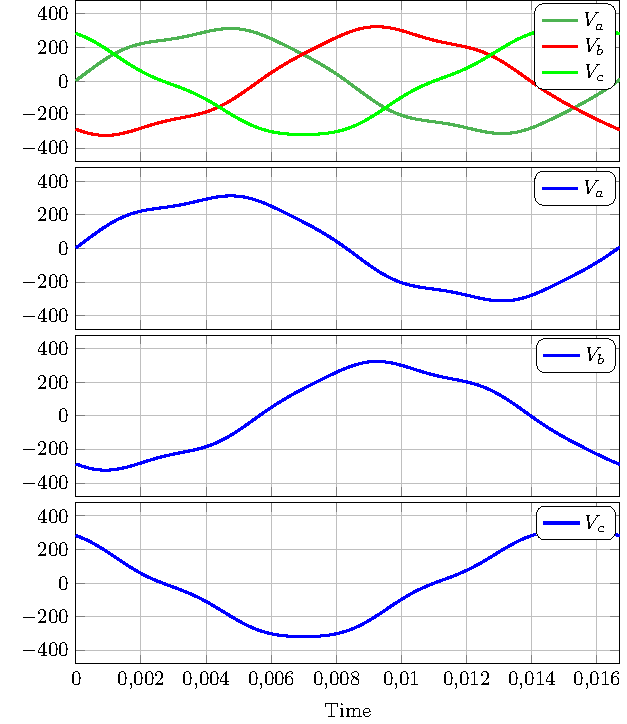
\includegraphics[width=\linewidth]{pictures/ex01}
\fonte{o autor -- \showfont}
\end{figure}


Por exemplo, na \figref{fig:ex01}, tem-se...

\begin{figure}
    \caption{Exemplo de aquisição}
    \label{fig:tek0009}
    \centering
    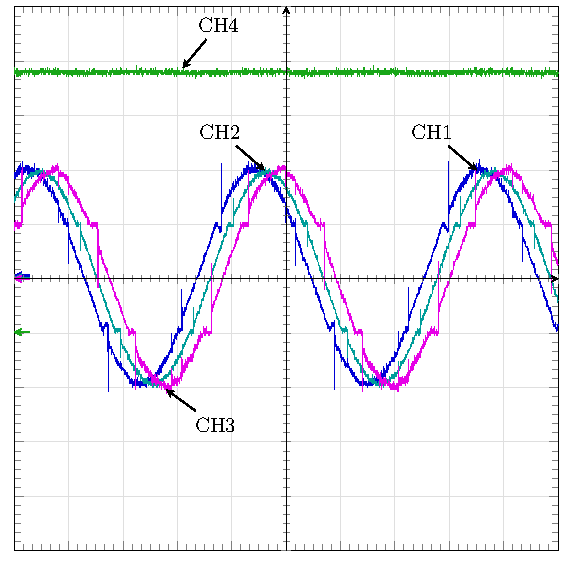
\includegraphics[width=0.9\linewidth]{pictures/tek0009}
    \fonte{o autor -- \showfont}
\end{figure}

Este documento e seu código-fonte são exemplos de referência de uso da classe
\textsf{abntex2} e do pacote \textsf{abntex2cite}. O documento
exemplifica a elaboração de trabalho acadêmico (tese, dissertação e outros do
gênero) produzido conforme a ABNT NBR 14724:2011 \emph{Informação e documentação
- Trabalhos acadêmicos - Apresentação}.

A expressão ``Modelo Canônico'' é utilizada para indicar que \abnTeX{} não é
modelo específico de nenhuma universidade ou instituição, mas que implementa tão
somente os requisitos das normas da ABNT. Uma lista completa das normas
observadas pelo \abnTeX{} é apresentada em \textcite{abntex2classe}.

Sinta-se convidado a participar do projeto \abnTeX{}! Acesse o site do projeto em
\url{http://abntex2.googlecode.com/}. Também fique livre para conhecer,
estudar, alterar e redistribuir o trabalho do \abnTeX{}, desde que os arquivos
modificados tenham seus nomes alterados e que os créditos sejam dados aos
autores originais, nos termos da ``The \LaTeX{} Project Public
License''\footnote{\url{http://www.latex-project.org/lppl.txt}}.

Encorajamos que sejam realizadas customizações específicas deste exemplo para
universidades e outras instituições --- como capas, folha de aprovação, etc.
Porém, recomendamos que ao invés de se alterar diretamente os arquivos do
\abnTeX{}, distribua-se arquivos com as respectivas customizações.
Isso permite que futuras versões do \abnTeX{}~não se tornem automaticamente
incompatíveis com as customizações promovidas. Consulte
\textcite{abntex2-wiki-como-customizar} par mais informações.

Este documento deve ser utilizado como complemento dos manuais do \abnTeX{}
\cite{abntex2classe,abntex2cite,abntex2cite-alf} e da classe \textsf{memoir}
\cite{memoir}.

Esperamos, sinceramente, que o \abnTeX{} aprimore a qualidade do trabalho que
você produzirá, de modo que o principal esforço seja concentrado no principal:
na contribuição científica.

Equipe \abnTeX{}

Lauro César Araujo




    % O comando \phantomsection é importante para a correta geração de links pelo hyperref.
\phantomsection

% O \chapter* usa um asterisco para que não seja numerado automaticamente, 
% caso seu orientador prefira assim. Se quiser numerado (ex: "Capítulo 2"), 
% use apenas \chapter{Fundamentação Teórica}.
\chapter{Fundamentação Teórica}
\label{ch:fundamentacao-teorica}

% ---
\section{Introdução ao Capítulo}
\label{sec:fund-intro}
% Escreva aqui um parágrafo introdutório que apresenta os objetivos e a estrutura deste capítulo.
% Ex: "Este capítulo estabelece a base conceitual para o presente trabalho, iniciando pela discussão
% sobre o direito à privacidade e o arcabouço legal da LGPD, passando pelas técnicas de
% anonimização de dados clínicos e concluindo com as métricas utilizadas para avaliar o
% balanço entre a proteção da privacidade e a utilidade dos dados para pesquisa."
% ---

% ---
\section{Privacidade e Proteção de Dados na Saúde: O Cenário da LGPD}
\label{sec:fund-lgpd}

\subsection{O Conceito de Privacidade na Era Digital}
\label{subsec:fund-privacidade}
Em uma das primeiras definições de privacidade, Samuel Warren e Louis Brandeis \cite{WarrenBrandeis1890} articularam a existência de um "direito a ser deixado em paz" (\textit{the right to be let alone}). O argumento era de que a proteção de pensamentos, sentimentos e emoções expressos por meio da escrita ou das artes contra plágio ou apropriação física não era um princípio da propriedade privada (sob o qual a propriedade intelectual é baseada), mas sim um direito a "inviolabilidade pessoal", e portanto não somente  as produções intelectuais ou artísticas, mas também as expressões casuais do dia a dia — pensamentos, emoções e ações - deveriam ser protegidas da exposição pública indesejada. Com isso, a privacidade foi estabelecida como um direito universal que não deriva de um contrato ou de uma relação de propriedade, mas sim como um princípio inerente à dignidade humana, lançando as bases para todo o debate futuro sobre o tema.

Décadas depois, já no início da era da computação, em \textit{Privacy and Freedom}, Alan Westin analisou como as novas tecnologias de vigilância e a capacidade de armazenamento e processamento de dados em computadores, criavam uma ameaça inédita à liberdade individual. Diante desse cenário, Westin formulou sua influente definição de privacidade como o direito de um indivíduo de determinar quando, como e em que medida as informações sobre si são comunicadas a terceiros \cite{Westin1967}. Essa noção, conhecida como "autodeterminação informativa", deslocou o foco de um direito passivo ao isolamento para um poder ativo de controle sobre o fluxo de dados pessoais. É este o princípio que constitui a base da Lei Geral de Proteção de Dados Pessoais (LGPD) brasileira \cite{Brasil2018lgpd}. A LGPD, ao estabelecer as bases legais para o tratamento de dados, como o consentimento informado e a finalidade legítima, materializa a visão de Westin: ela não proíbe o uso de dados, mas o regulamenta para garantir que o titular mantenha o controle sobre suas informações, transformando um princípio filosófico em um direito legal e aplicável.

Outra definição fundamental para este trabalho, que avança em relação à noção de controle individual, é a de Integridade Contextual, proposta por Helen Nissenbaum. Em sua obra \textit{Privacy in Context}, a autora argumenta que a privacidade não é simplesmente sobre manter informações secretas, mas sim sobre garantir que o fluxo de informações pessoais siga as normas esperadas para um determinado contexto social \cite{Nissenbaum2009}. A violação da privacidade ocorre quando essas normas são quebradas. Nissenbaum modela essas normas a partir de três parâmetros: os atores (quem envia, quem recebe), os atributos (o tipo de informação) e os princípios de transmissão (as regras que governam o fluxo). O contexto da saúde pode ser um exemplo: um paciente (ator) espera que seu diagnóstico (atributo) seja compartilhado com outro especialista (ator) sob um princípio de confidencialidade, mas ficaria chocado se o mesmo dado fosse vendido a uma empresa de marketing, pois isso violaria as normas contextuais.

% Para a presente pesquisa, o conceito de Nissenbaum é crucial, pois justifica a anonimização não como uma perda de controle, mas como uma mudança de contexto: ao anonimizar os dados clínicos, removemos os atores originais (pacientes) para adequar a informação a um novo contexto — o da pesquisa científica —, com novos atores (pesquisadores) e novos princípios de transmissão (uso para o bem comum), mantendo assim a integridade do fluxo informacional.

Finalmente, a discussão sobre privacidade na era digital seria incompleta sem analisar a lógica econômica que a desafia em sua essência. Em sua obra \textit{A Era do Capitalismo de Vigilância}, a economista Shoshana Zuboff argumenta que a massiva coleta de dados por empresas de tecnologia não é um simples efeito colateral, mas a fundação de uma nova forma de mercado \cite{Zuboff2019}. Nesse modelo, as experiências humanas são tratadas como matéria-prima gratuita e processadas como "excedente comportamental". Este excedente é utilizado para fabricar "produtos de predição", que são vendidos em novos mercados com o objetivo de antecipar e até mesmo influenciar o comportamento dos usuários. Essa lógica econômica choca-se frontalmente com as definições anteriores: ela torna o ideal de controle individual de Westin uma ilusão, ao operar por meio da extração massiva e da ofuscação, e viola sistematicamente a integridade contextual de Nissenbaum, ao remover os dados de seu contexto original para alimentar outros mercados de futuros comportamentais. Com essa nova lógica mercadológica, a questão da privacidade se transforma de uma violação individual para um desafio sistêmico ao qual a legislação precisa se adaptar. A resposta legal começa por categorizar e definir precisamente o objeto de proteção, o que nos leva à distinção fundamental entre o dado pessoal e o dado sensível.

\subsection{O Dado Pessoal e o Dado Sensível}
\label{subsec:fund-dados-sensiveis}

O Art. 5º, inciso I, da LGPD \cite{Brasil2018lgpd} define dado pessoal como "informação relacionada a pessoa natural identificada ou identificável". Essa definição é propositalmente ampla, abrangendo não apenas dados que apontam diretamente para um indivíduo, como nome completo ou CPF, mas também informações que, isoladamente ou em combinação com outras, podem levar à identificação de uma pessoa. Exemplos incluem endereços IP, dados de geolocalização, ou mesmo uma combinação de atributos como profissão, cidade e idade.

No inciso seguinte do mesmo artigo (Art. 5º, II), a LGPD qualifica o dado sensível, um subconjunto especial de dados pessoais que, devido à sua natureza, requer um nível mais elevado de proteção. Entre as informações destacadas como dados sensíveis pela legislação, estão "dados referentes à saúde" e "dados genéticos ou biométricos". A inclusão desses tipos de dados na categoria de sensíveis reflete o reconhecimento de que sua exposição pode levar a discriminação, estigmatização ou outros danos significativos ao titular. Por exemplo, a divulgação não autorizada de um diagnóstico médico pode afetar a vida pessoal e profissional de um indivíduo, enquanto dados genéticos podem revelar predisposições a certas doenças que podem impactar decisões de seguro ou emprego.

A definição de dado sensível como posta na legislação (por meio de exemplificação) não é exaustiva, e que para determinar um dado como sensível é essencial verificar o contexto de sua utilização e sua relação com outras informações disponíveis. Dessa forma, deve-se admitir que outros dados, não explicitamente mencionados como sensíveis, podem ser considerados como tal a depender do uso que se faz deles e sua potencialidade de se tornar instrumentos de discriminação ou violação de direitos fundamentais \cite{TefferViola2020}. Isso reforça a necessidade de um cuidado redobrado no tratamento de dados pessoais na área da saúde, que mesmo quando não categorizados formalmente como sensíveis, podem revelar aspectos íntimos da vida dos pacientes.

\subsection{Pilares da LGPD: Consentimento e Transparência}
\label{subsec:fund-consentimento}

O Art. 7º da LGPD é dedicado às hipóteses que autorizam o tratamento de dados pessoais. Entre essas, o inciso I destaca tutela especial para o consentimento do titular dos dados - mesmo que esta não seja a única base legal para o uso de dados. O consentimento, conforme definido no Art. 5º, inciso IX, deve ser fornecido de forma livre, informada e inequívoca, garantindo que o titular compreenda plenamente as implicações do tratamento de seus dados. Isso inclui a finalidade específica para a qual os dados serão utilizados, o período de armazenamento e os direitos do titular em relação aos seus dados. Dessa forma, entende-se que o consentimento é restritivo, de modo que o agente não pode estender a autorização concedida para outras finalidades não previstas inicialmente, e que o titular pode revogar o consentimento a qualquer momento, conforme previsto no Art. 8º da LGPD.

Para \citeonline{TefferViola2020}, \textit{Livre} significa que o titular pode escolher a utilização de seus dados sem intervenções ou pressões externas que viciem o consentimento por meio de assimetria entre as partes. \textit{Informado} implica que o titular deve ter a sua disposição informações suficientes e acessíveis para avaliar a forma como seus dados serão tratados e os riscos e implicações do processo, levando em conta a assimetria técnica e informacional entre as partes. Já \textit{inequívoco} sugere que o consentimento deve ser expresso de maneira clara, sem ambiguidades, seja por meio de uma ação afirmativa ou declaração explícita, de modo que o ônus da prova de que o consentimento foi obtido de forma adequada recai sobre o agente de tratamento.

O cumprimento desses requisitos granulares, somado à necessidade de gerenciar a revogação do consentimento, impõe um significativo ônus operacional e burocrático às organizações. Essa definição rigorosa reflete a preocupação da LGPD em garantir que o titular mantenha o controle sobre seus dados pessoais, alinhando-se com o conceito de autodeterminação informativa de Westin discutida na seção anterior.

Apesar de que o consentimento não seja a única base legal para o tratamento de dados, ele é especialmente relevante no contexto de dados sensíveis, que requerem tutela especial. O Art. 11 da LGPD estabelece que o tratamento de dados sensíveis somente poderá ocorrer com o consentimento específico e destacado do titular, salvo em situações excepcionais previstas na lei, como cumprimento de obrigação legal ou regulatória, proteção da vida ou da incolumidade física do titular ou de terceiros, ou para a tutela da saúde, exclusivamente em procedimento realizado por profissionais de saúde, serviços de saúde ou autoridade sanitária.
Essas exceções reconhecem que há circunstâncias em que o tratamento de dados sensíveis é necessário para proteger interesses públicos ou direitos fundamentais, mesmo sem o consentimento do titular.

Como complemento ao consentimento, a LGPD estabelece o princípio da transparência como um de seus pilares fundamentais, conforme o Art. 6º, inciso VI. Este princípio garante aos titulares o acesso a "informações claras, precisas e facilmente acessíveis" sobre como seus dados são tratados. Na prática, a transparência é a ferramenta que viabiliza o consentimento verdadeiramente "informado". Sem que as organizações comuniquem abertamente quais dados são coletados, para qual finalidade e por quanto tempo, o titular não possui as condições necessárias para consentir de forma livre e consciente. Portanto, a combinação do consentimento (a ação do titular) com a transparência (o dever do controlador) busca reequilibrar a relação assimétrica entre as partes, fomentando a confiança no tratamento de dados pessoais.

\subsection{O Tratamento de Dados para Fins de Pesquisa na LGPD}
\label{subsec:fund-pesquisa-lgpd}

Como destacado na seção anterior, o tratamento de dados pessoais, como os dados clínicos, é fortemente regulado pela LGPD, exigindo o consentimento explícito do titular. No entanto, a lei também reconhece a importância do avanço científico e tecnológico para a sociedade, estabelecendo exceções específicas para o uso de dados pessoais sem consentimento em determinados contextos de pesquisa. Em seu Art. 7º, inciso IV, a lei estabelece uma base legal específica que autoriza o tratamento de dados pessoais "para a realização de estudos por órgão de pesquisa", dispensando a necessidade de outras bases legais como o consentimento \cite{Brasil2018lgpd}. Conforme o Art. 5º, XVIII, a definição de "órgão de pesquisa" é ampla, incluindo entidades da administração pública e organizações privadas sem fins lucrativos que tenham como missão institucional a pesquisa básica ou aplicada.

A LGPD é ainda mais específica ao tratar do uso de dados sensíveis no contexto da pesquisa científica. O Art. 11, inciso II, prevê que o tratamento de dados sensíveis pode ocorrer sem o consentimento do titular "para a realização de estudos por órgão de pesquisa, garantida, sempre que possível, a anonimização dos dados pessoais sensíveis" \cite{Brasil2018lgpd}. Essa disposição reconhece que a pesquisa científica muitas vezes depende do acesso a dados sensíveis para gerar conhecimento que pode beneficiar a sociedade como um todo. Ainda assim, a lei estabelece uma diretriz clara que preza pela desvinculação completa entre os dados e os indivíduos, buscando minimizar os riscos de violação de privacidade.

A anonimização dos dados, como especificada na LGPD, é a principal ferramenta para equilibrar a proteção da privacidade dos titulares dos dados com a necessidade de acesso a informações sensíveis para fins de pesquisa e desenvolvimento científico. Essa salvaguarda impões também um desafio técnico significativo para as instituições de pesquisa, que devem ser mais cautelares na forma como coletam, armazenam e processam dados sensíveis a fim de garantir uma anonimização que reduza o risco de reidentificação dos indivíduos ao mesmo tempo em que preserva a utilidade dos dados para análise científica.

\subsection{Anonimização vs. Pseudonimização sob a Ótica da Lei}
\label{subsec:fund-anon-pseudo}
% Apresente a definição técnica e jurídica de cada termo, deixando claro por que a
% anonimização efetiva é o objetivo para dispensar o consentimento.

Tratando-se de um instrumento essencial para a proteção da privacidade, a anonimização é um conceito que ganha atenção especial na LGPD. Conforme o Art. 5º, inciso XI, é definida como a "utilização de meios técnicos razoáveis e disponíveis no momento do tratamento, por meio dos quais um dado perde a possibilidade de associação, direta ou indireta, a um indivíduo". Ainda, a lei também faz a distinção com a pseudonimização, definida como um tratamento de segurança que, por meio da separação de informações, faz com que um dado perca a possibilidade de associação direta a um indivíduo, exceto pelo uso de informação adicional mantida separadamente pelo controlador \cite[Art. 13, § 4º]{Brasil2018lgpd}. Nesse sentido, determina-se que apesar de ambas as técnicas visarem a proteção da privacidade, a anonimização é um processo mais robusto, pois remove permanentemente a possibilidade de reidentificação, enquanto a pseudonimização apenas dificulta essa associação, mas não a elimina completamente.

Como consequência dessa distinção, entende-se que o dado pseudoanonimizado é identificável, e portanto continua sendo considerado um dado pessoal sob a LGPD cujo tratamento requer uma base legal, como o consentimento do titular. Já o dado anonimizado, por perder a possibilidade de associação a um indivíduo, deixa de ser considerado um dado pessoal e, portanto, pode ser tratado sem a necessidade de consentimento, desde que a anonimização seja efetiva e irreversível. Isso significa que, uma vez anonimizado, o conjunto de dados pode ser utilizado para pesquisa e outras finalidades sem as restrições impostas pela LGPD. Para o escopo deste trabalho, o foco será na anonimização, buscando um método de tratamento de dados que dissocie de forma irreversível os dados clínicos de seus titulares.

% ---
\section{O Valor dos Dados Clínicos para Pesquisa e Inovação}
\label{sec:fund-valor-dados}

\subsection{A Importância do Big Data na Saúde}
\label{subsec:fund-bigdata}
% Apresente exemplos de como grandes volumes de dados de saúde podem acelerar descobertas,
% melhorar diagnósticos e otimizar a gestão em saúde pública.

\subsection{Dados Estruturados vs. Dados Não Estruturados}
\label{subsec:fund-dados-estruturados}
% Defina e exemplifique os dois tipos de dados no contexto clínico (ex: exames laboratoriais vs. notas de evolução).
% Discuta os desafios e as oportunidades de cada um para a anonimização e análise.
% ---

% ---
\section{Métodos e Técnicas de Anonimização de Dados}
\label{sec:fund-metodos-anon}

\subsection{Abordagens Iniciais: Generalização e Supressão (k-Anonimato)}
\label{subsec:fund-k-anonimato}
% Explique o conceito de k-Anonimato, como ele funciona na prática (agrupando indivíduos) e
% discuta suas principais vulnerabilidades, como o ataque de homogeneidade.

\subsection{Refinando a Proteção: l-Diversidade e t-Proximidade}
\label{subsec:fund-l-diversidade}
% Descreva como a l-Diversidade e a t-Proximidade surgiram para corrigir as falhas
% do k-Anonimato, adicionando requisitos sobre a variedade dos dados sensíveis nos grupos.

\subsection{Técnicas de Randomização e Perturbação}
\label{subsec:fund-randomizacao}
% Apresente brevemente outras técnicas, como a adição de ruído aleatório, e discuta
% seus prós e contras em relação à utilidade dos dados.

\subsection{Privacidade Diferencial: O Padrão-Ouro de Garantia Matemática}
\label{subsec:fund-privacidade-diferencial}
% Explique de forma conceitual o que é a Privacidade Diferencial. Foque na ideia de que a
% saída de uma consulta é praticamente a mesma com ou sem os dados de um indivíduo específico.
% Mencione o papel do parâmetro epsilon ($\epsilon$) no controle do balanço privacidade-utilidade.
% Lembre-se de usar o modo matemático para o epsilon, assim: $\epsilon$.
% ---

% ---
\section{Métricas de Avaliação: O Balanço entre Privacidade e Utilidade}
\label{sec:fund-metricas}

\subsection{Avaliação do Risco de Reidentificação (Métricas de Privacidade)}
\label{subsec:fund-metricas-privacidade}
% Descreva como se pode quantificar o risco de um indivíduo ser reidentificado em um dataset
% anonimizado. Apresente algumas métricas ou modelos de risco.

\subsection{Avaliação da Utilidade dos Dados Anonimizados (Métricas de Qualidade)}
\label{subsec:fund-metricas-utilidade}
% Detalhe as duas abordagens principais para medir a qualidade/utilidade dos dados:
% 1. Similaridade estatística (comparação de distribuições, correlações, etc.).
% 2. Performance em tarefas de Machine Learning (comparando a performance de um modelo
%    treinado nos dados originais vs. nos dados anonimizados).
% ---

% ---
\section{Síntese da Fundamentação e Escolha da Abordagem}
\label{sec:fund-sintese}
% Feche o capítulo com um ou dois parágrafos que resumam o que foi apresentado e, o mais importante,
% justifique quais técnicas e métricas discutidas aqui serão empregadas na parte prática do seu TCC.
% Isso cria a ponte perfeita para o seu próximo capítulo (Metodologia/Desenvolvimento).
% ---

    % PARTE
    \ifforcedinclude\else\part{\lang{Implementation}{Implementação}}\fi
    \label{segunda_parte}


    % Finaliza a parte no bookmark do PDF para que se inicie o bookmark na raiz
    % e adiciona espaço de parte no Sumário
    \phantompart

    % Conclusão (outro exemplo de capítulo sem numeração e presente no sumário)
    
% The \phantomsection command is needed to create a link to a place in the document that is not a
% figure, equation, table, section, subsection, chapter, etc.
% https://tex.stackexchange.com/questions/44088/when-do-i-need-to-invoke-phantomsection
\phantomsection

% ---
\chapter{\lang{Final Remarks}{Considerações Finais}}
\phantomsection

    Lipsum me [31-33]



    % ELEMENTOS PÓS-TEXTUAIS
    \postextual
    \setlength\beforechapskip{0pt}
    \setlength\midchapskip{15pt}
    \setlength\afterchapskip{15pt}

    % Referências bibliográficas
    \begingroup
        % https://tex.stackexchange.com/questions/163559/how-to-modify-line-spacing-per-entry-of-bibliography
        % https://tex.stackexchange.com/questions/19105/how-can-i-put-more-space-between-bibliography-entries-biblatex
        \setlength\bibitemsep{\baselineskip}
        \advisor{}{\linespread{1.18}\selectfont}

        % https://tex.stackexchange.com/questions/17128/using-bibtex-to-make-a-list-of-references-without-having-citations-in-the-body
        % \nocite{*}
        \printbibliography[title=\lang{REFERENCES}{REFERÊNCIAS}]
    \endgroup

    % INDICE REMISSIVO
    \ifforcedinclude\else
        \phantompart
        \printindex
    \fi

\end{document}

